\documentclass{article}
\usepackage{titling}
\newcommand{\subtitle}[1]{%
  \posttitle{%
    \par\end{center}
    \begin{center}\large#1\end{center}
    \vskip0.5em}%
}
\usepackage{longtable}
\usepackage{epsfig}
\usepackage{amsmath}
\usepackage[linesnumbered,boxruled,vlined]{algorithm2e}
\newcommand{\BigO}[1]{\ensuremath{\operatorname{O}\bigl(#1\bigr)}}
\textwidth 6in
\addtolength{\oddsidemargin}{-0.5in}
\textheight 9in
\addtolength{\topmargin}{-0.5in}
\setlength{\parindent}{0pt}
\setlength{\parskip}{0.5cm}
\topskip 0.0in
%\pagestyle{empty}

\begin{document}
\title{CS315A : GROUP 05}
\subtitle{\textbf{SOCIAL NETWORKING}}
\author{
  Arihant Kumar Jain\\
  \texttt{11147}\\  
  \texttt{arikj@iitk.ac.in}\\
  \texttt{IITKanpur}
  \and
  Ashok Kumar\\
  \texttt{11164}\\
  \texttt{ashokrm@iitk.ac.in}\\
  \texttt{IITKanpur}
  \and
  Sangharsh Aglave\\
  \texttt{11643}\\
  \texttt{saglave@iitk.ac.in}\\
  \texttt{IITKanpur}
} 
%\date{January 08, 2014}
\date{\today}
\newcommand{\sus}[2]{$#1_{#2}$}
\maketitle
\newpage
%\tableofcontents
\newpage

\centerline{\textbf{Abstract}}

\section{Introduction}

\section{Approach}
The social network designed by us can be modelled in six entity-relationship digrams which are described in detail as follows:
\subsection{User - User relation}
\begin{figure}[h]
\centering
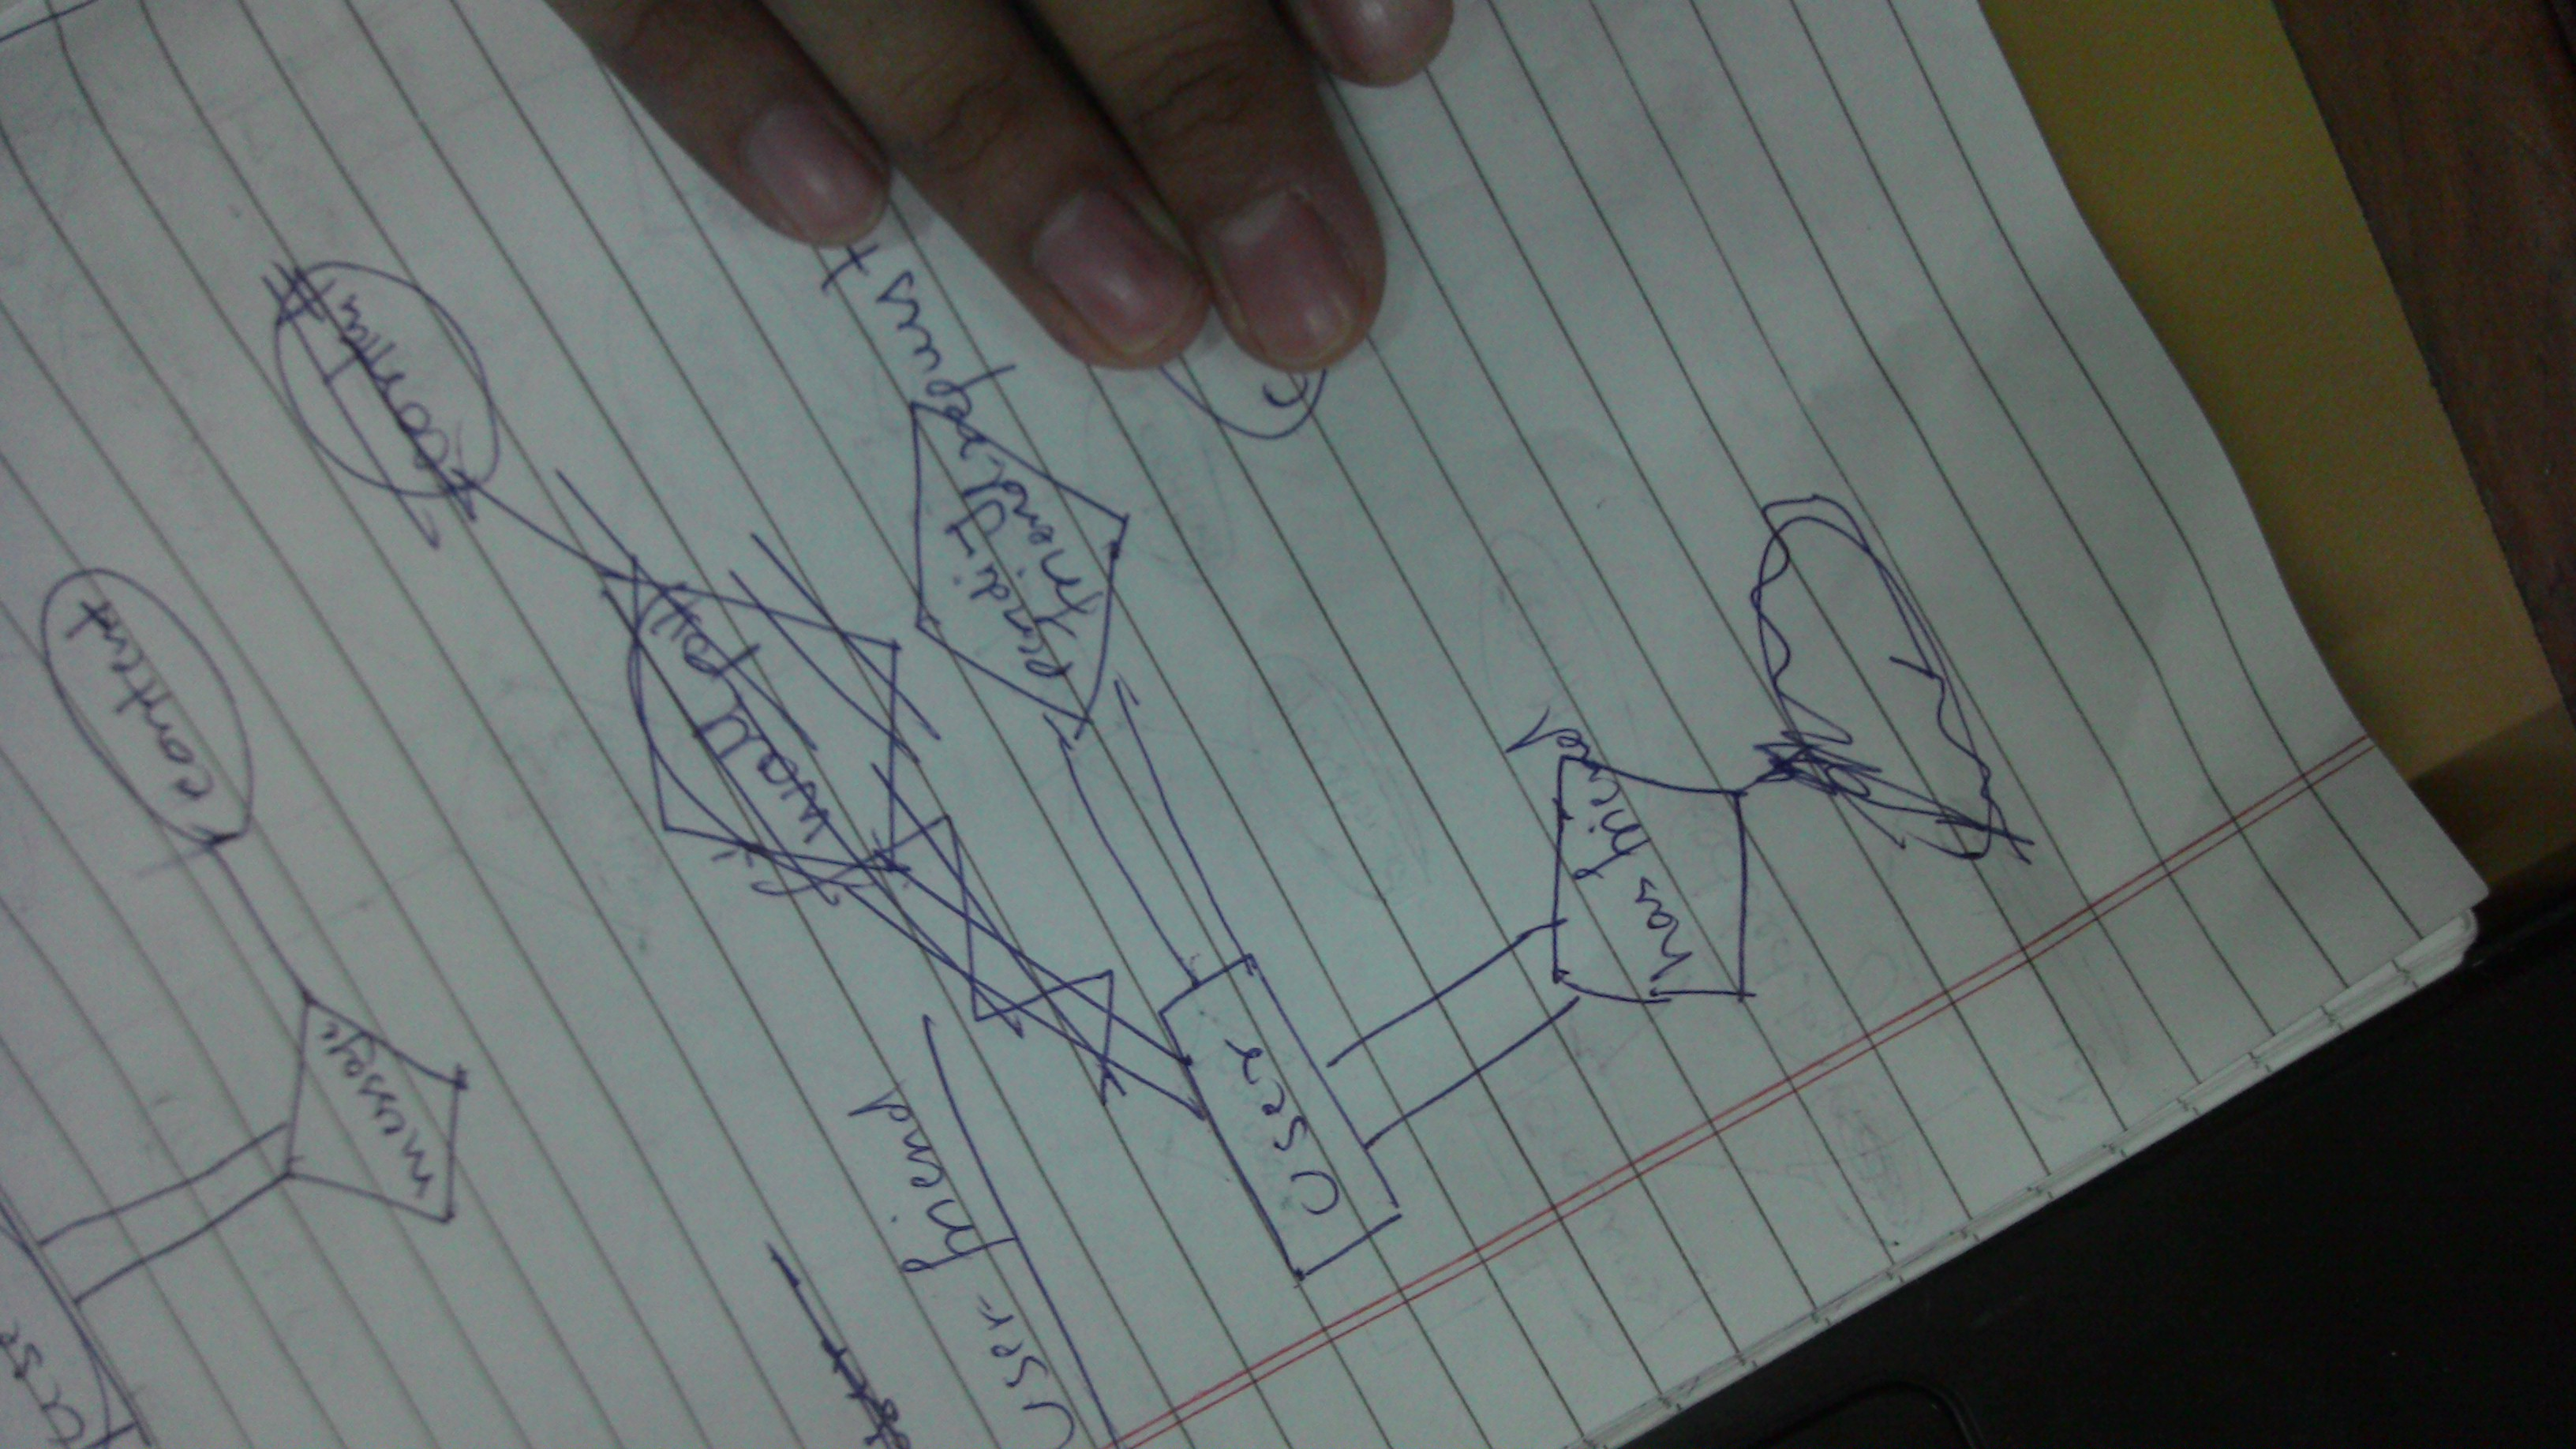
\includegraphics[scale=0.2]{fig1.jpg}
\caption{User - User relation}
\label{fig1}
\end{figure}
This relation determines how a user is related to other users in the network. There are two ways:
\begin{itemize}
\item \textbf{pending friend request:} If one user(say,A) sends friend request to other user(say,B), until the user B accepts the request, both users share the \textbf{pending friend request} relation as shown in the \ref{fig1}.
\item \textbf{Friends:} If user B accepts the friend request of user A, then the relationship between them change from pending friends to friends. 
\end{itemize}

\subsection{User - Page relation}
\begin{figure}[h]
\centering
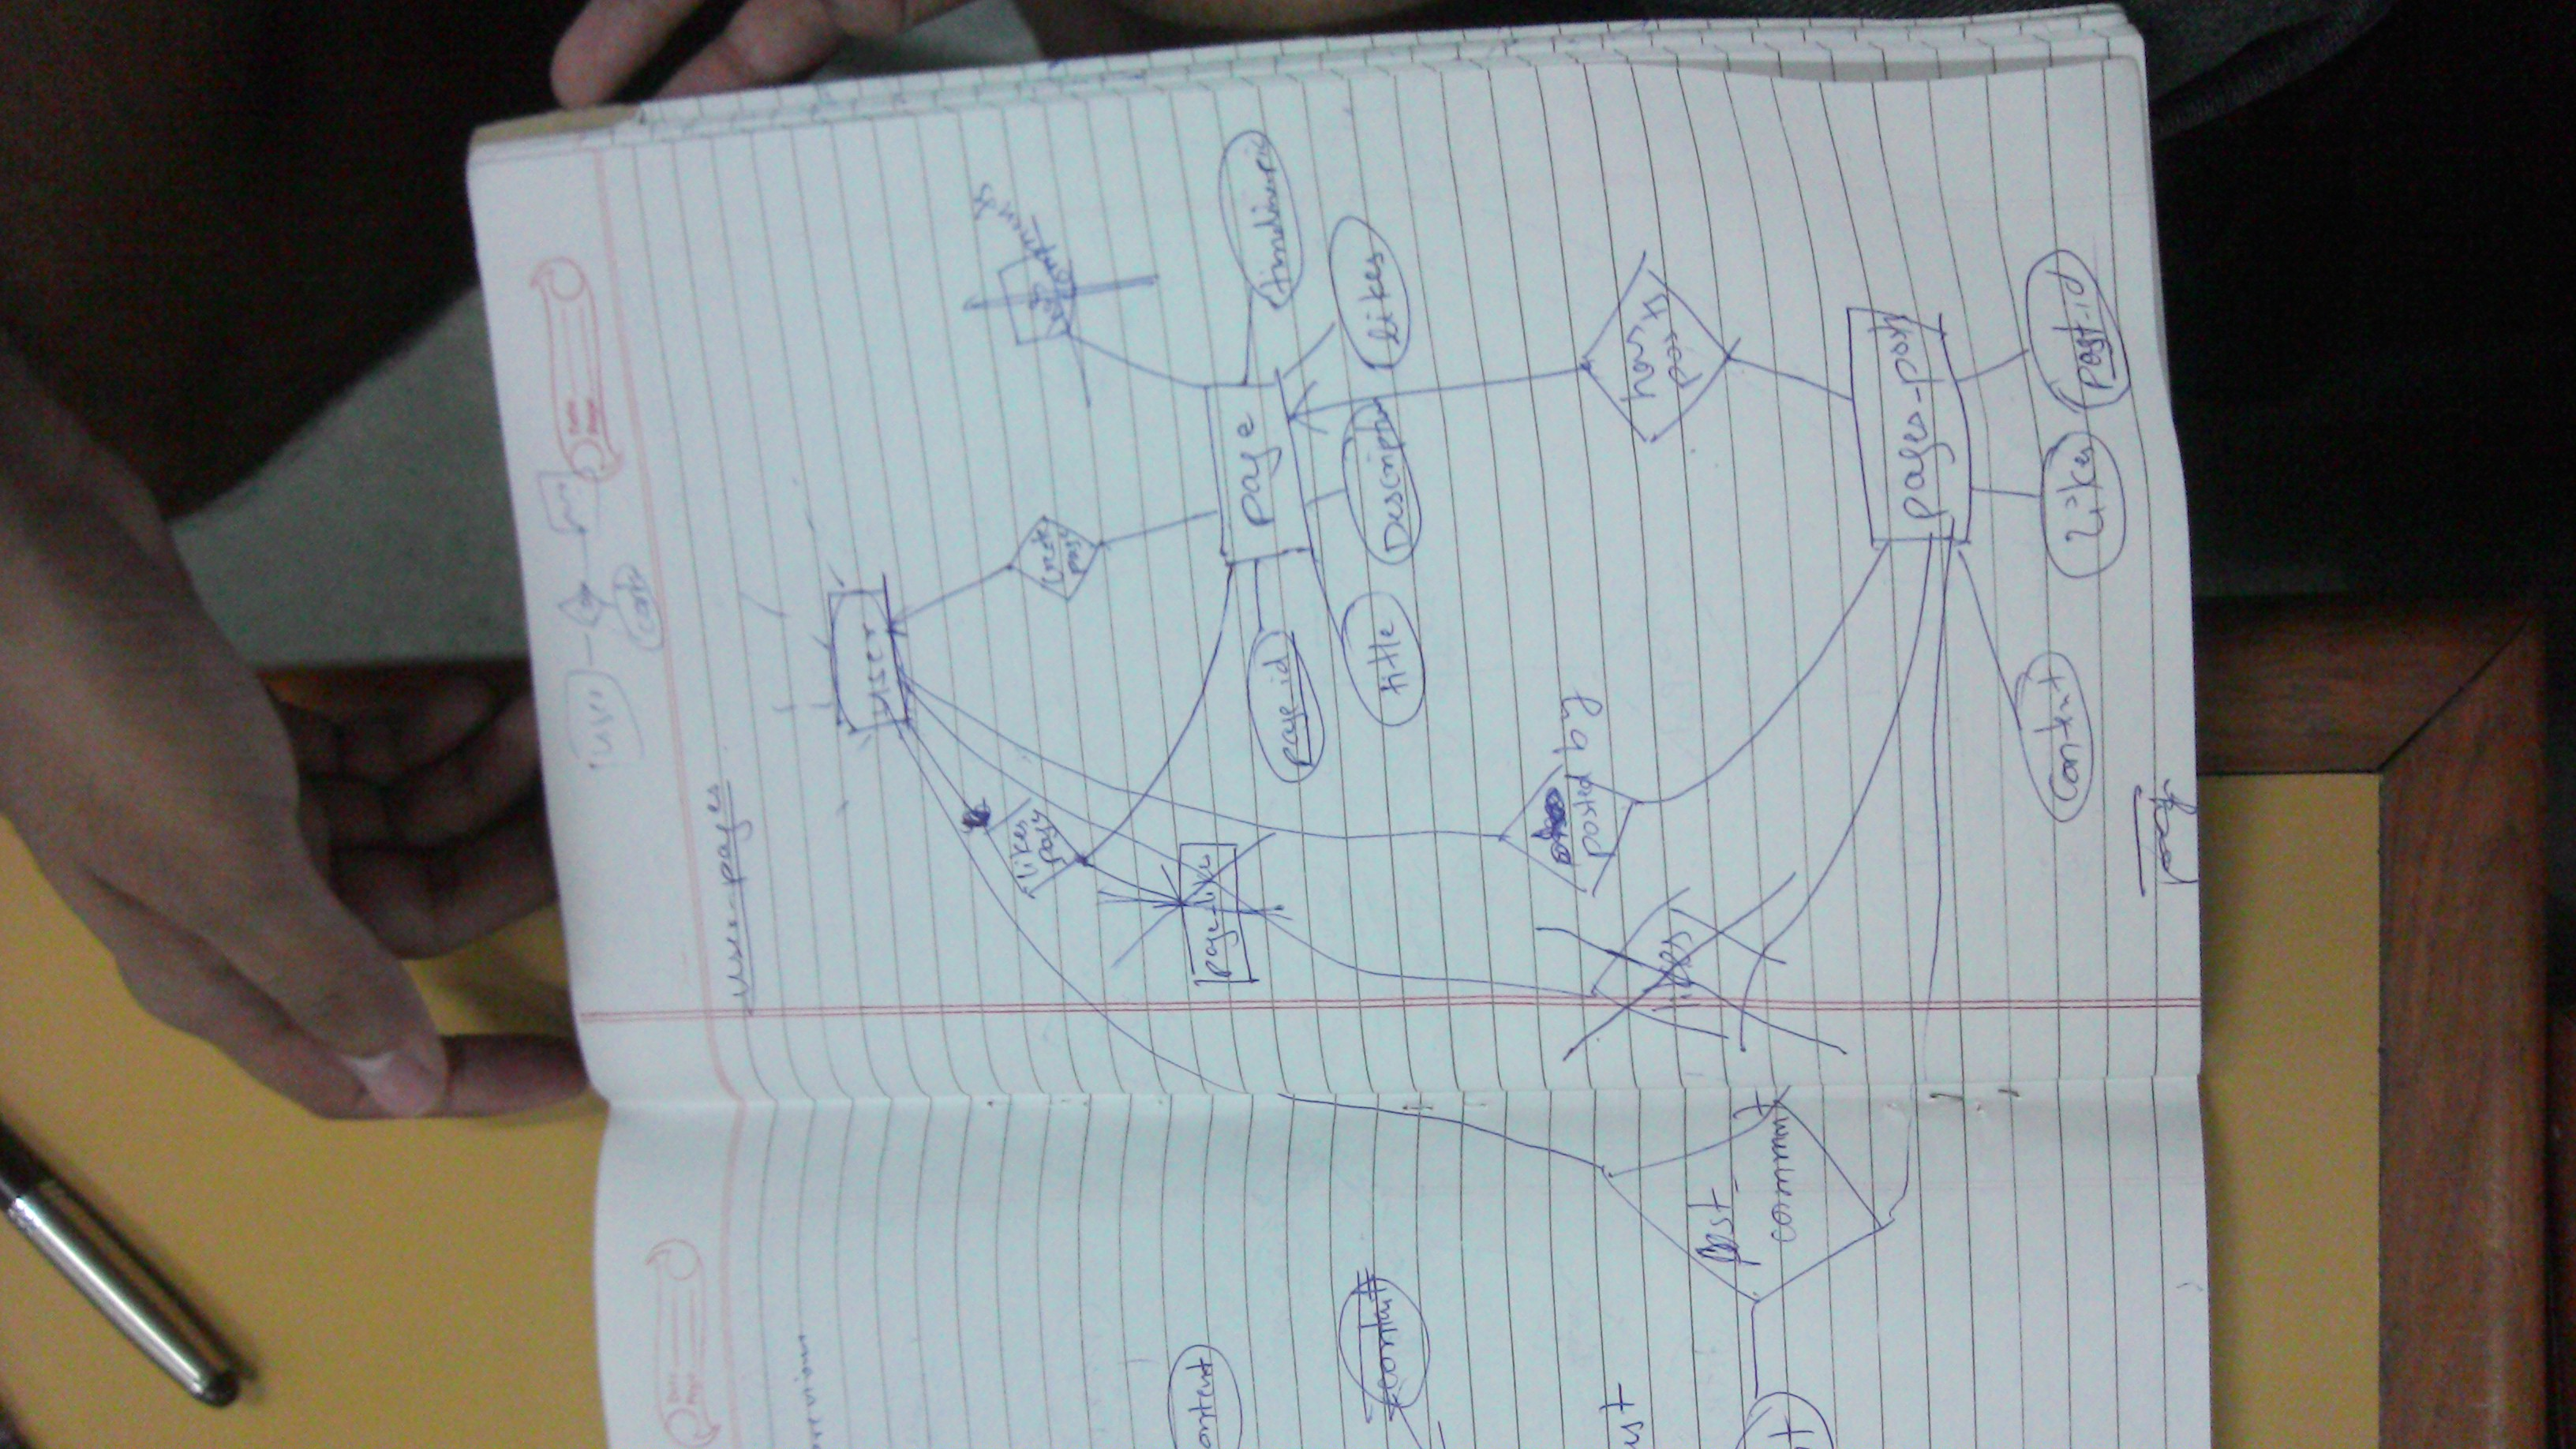
\includegraphics[scale=0.2]{fig2.jpg}
\caption{User - Page relation}
\label{fig2}
\end{figure}
Just as each user has a profile, a public page can be created for celebrites, organisations, and other entities. Unlike, user-profile, these pages are public, i.e., they are visible to every user. Users can post and read posts from a page once they like them. Users can be related to a page in following ways:
\begin{itemize}
\item \textbf{Create page:} User can create new pages with attributes like title, description, timeline picture etc.
\item \textbf{Like page:} User can like any number of pages of their interest and start reading and writing posts on the page.
\item \textbf{Page posts:} Each page can have multiple posts by different users and users can even comment on the post by other users.
\end{itemize}

\subsection{User - Group relation}
\begin{figure}[h]
\centering
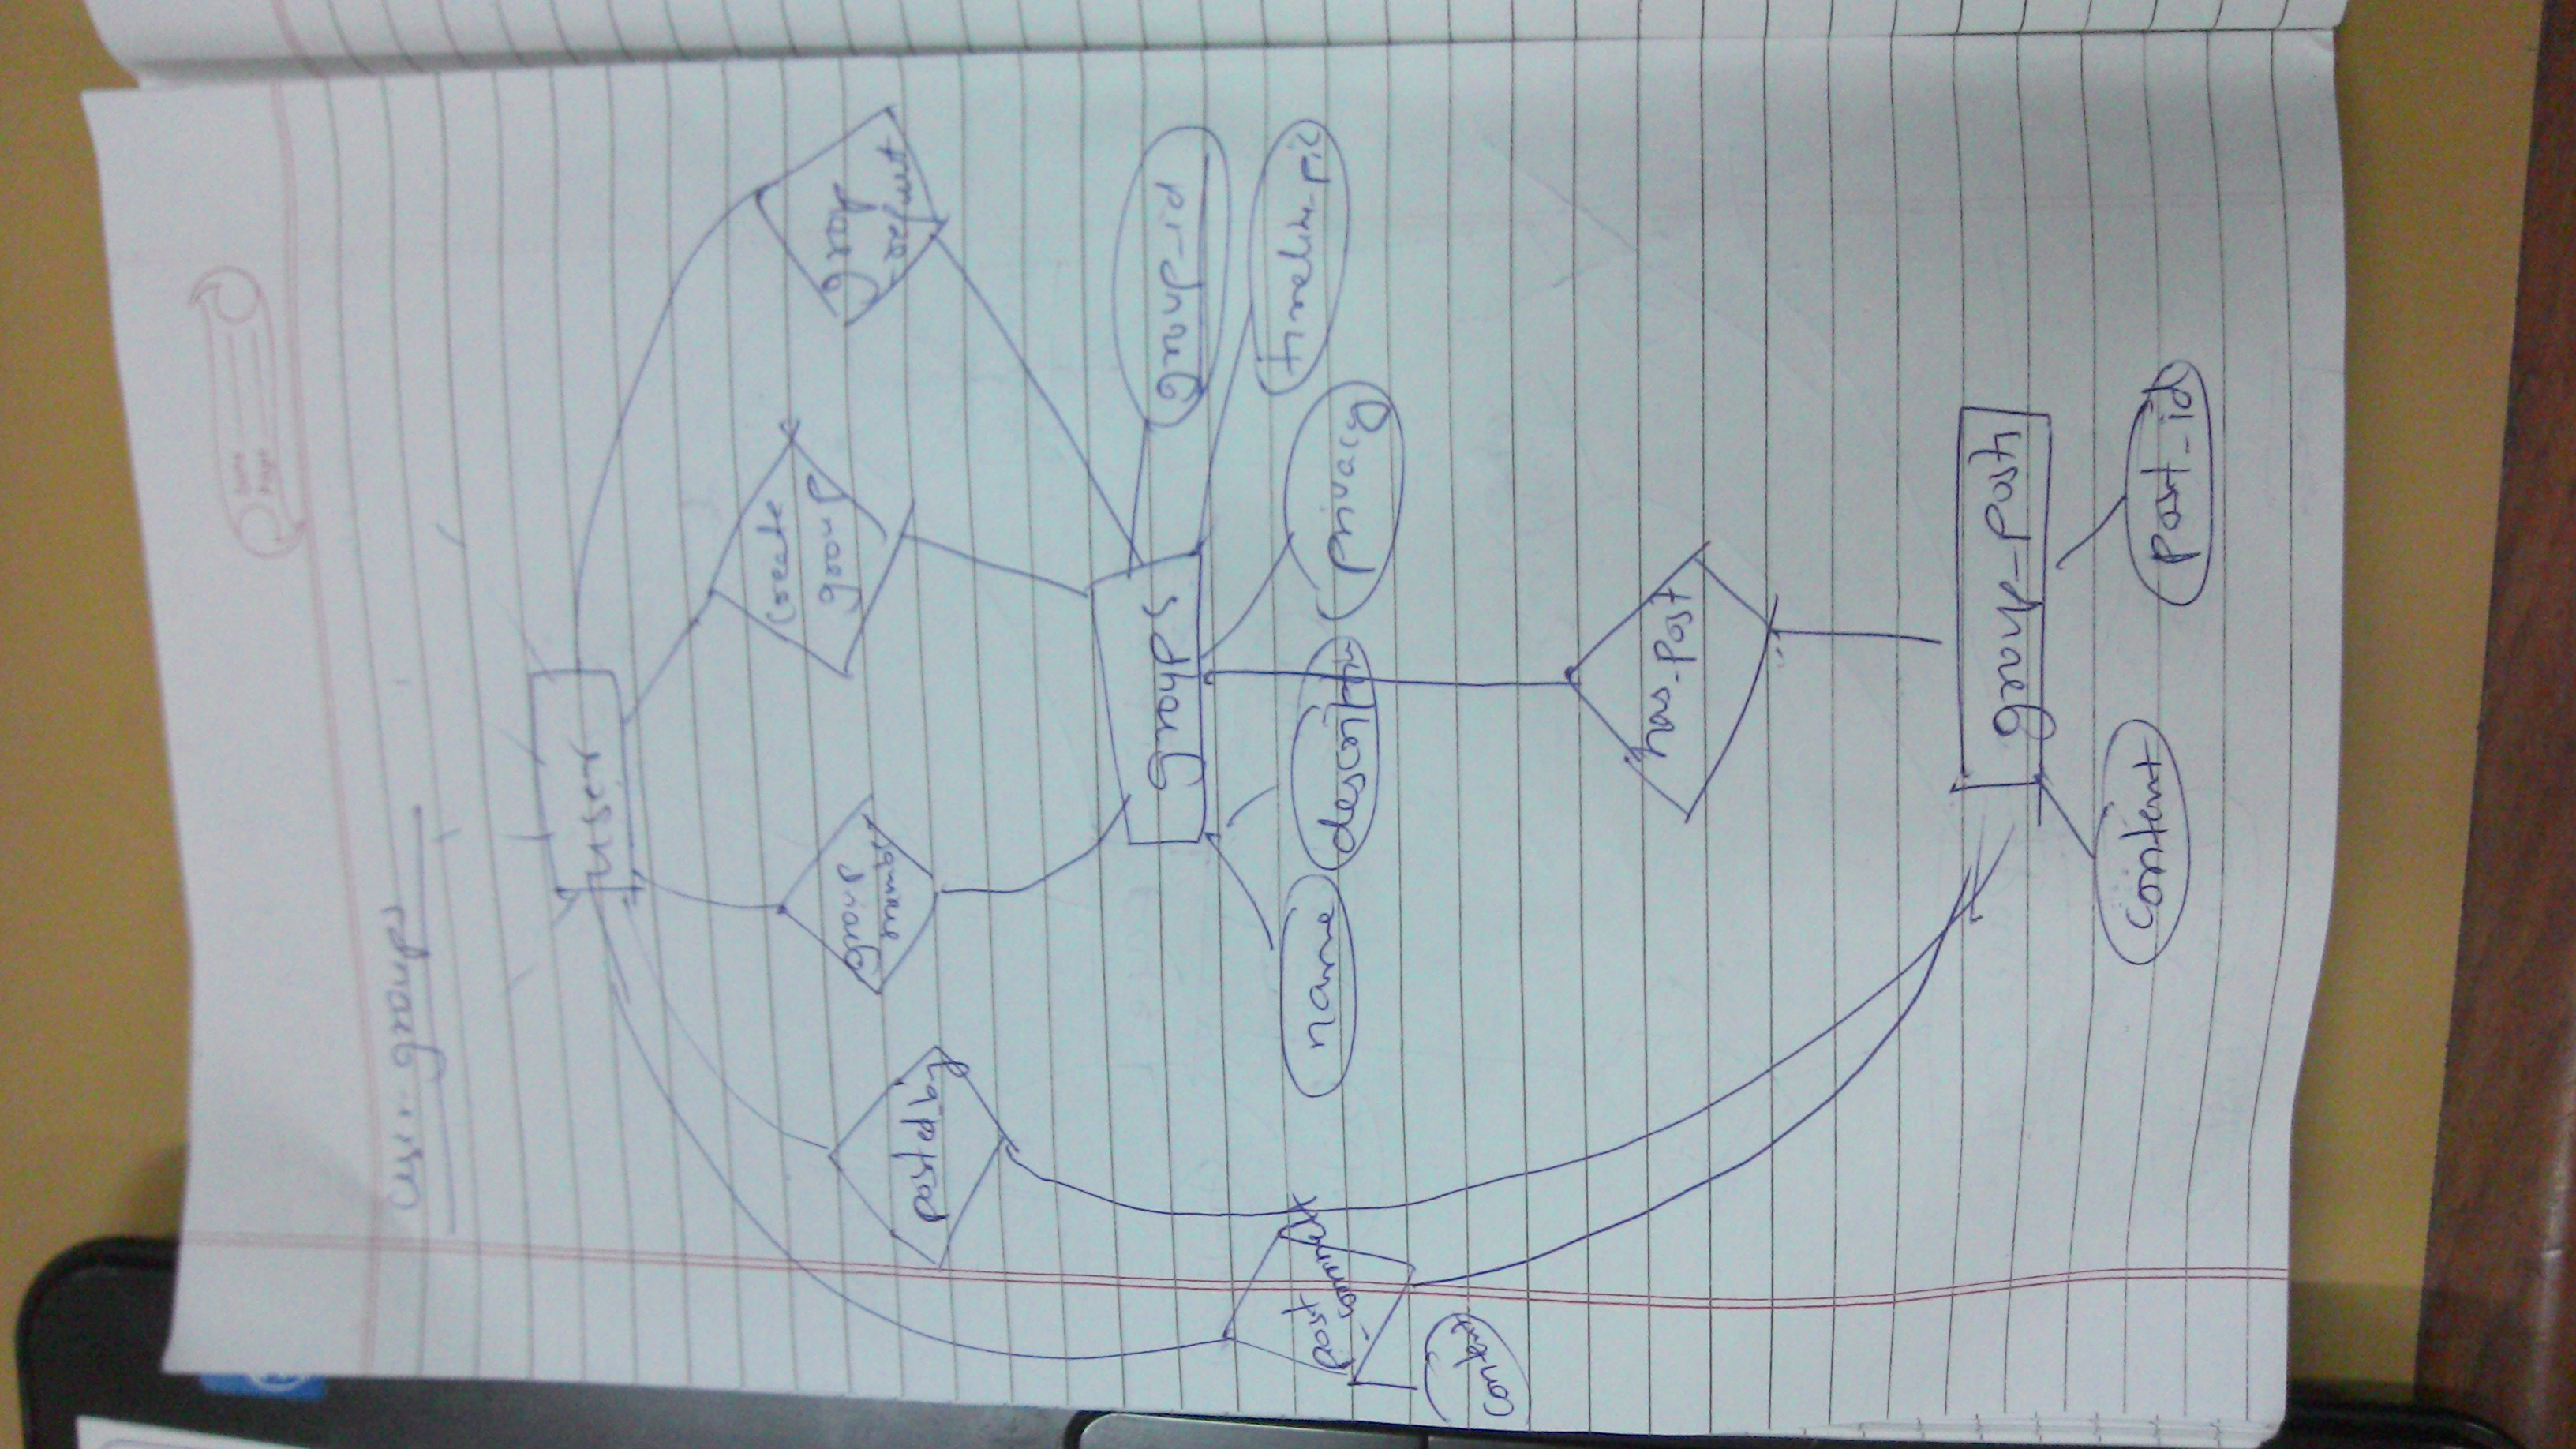
\includegraphics[scale=0.2]{fig3.jpg}
\caption{User - Group relation}
\label{fig3}
\end{figure}
Pages are designed to be the profiles for entities, groups are the place for small group communication and for people to share their common interests and express their opinion. When a new group is created by a user, he/she can decide whether to make it publicly available for anyone to join, or require his/her approval for members to join. The relationship between users and groups are described below:
\begin{itemize}
\item \textbf{Create group:} A user can create new groups which can be made public or private as described above. Groups will have attributes like title, description, timeline picture, privacy etc.
\item \textbf{Members:} If a group is public, users can directly become its member. But, if it is private, then a request will be send from the user to the creator of the group. It is upto the creator whether to allow the user to join or not.
\item \textbf{Group posts:} Only members of groups are allowed to view the content and write new posts in the group.
\end{itemize}
\subsection{User - Question relation}
\begin{figure}[h]
\centering
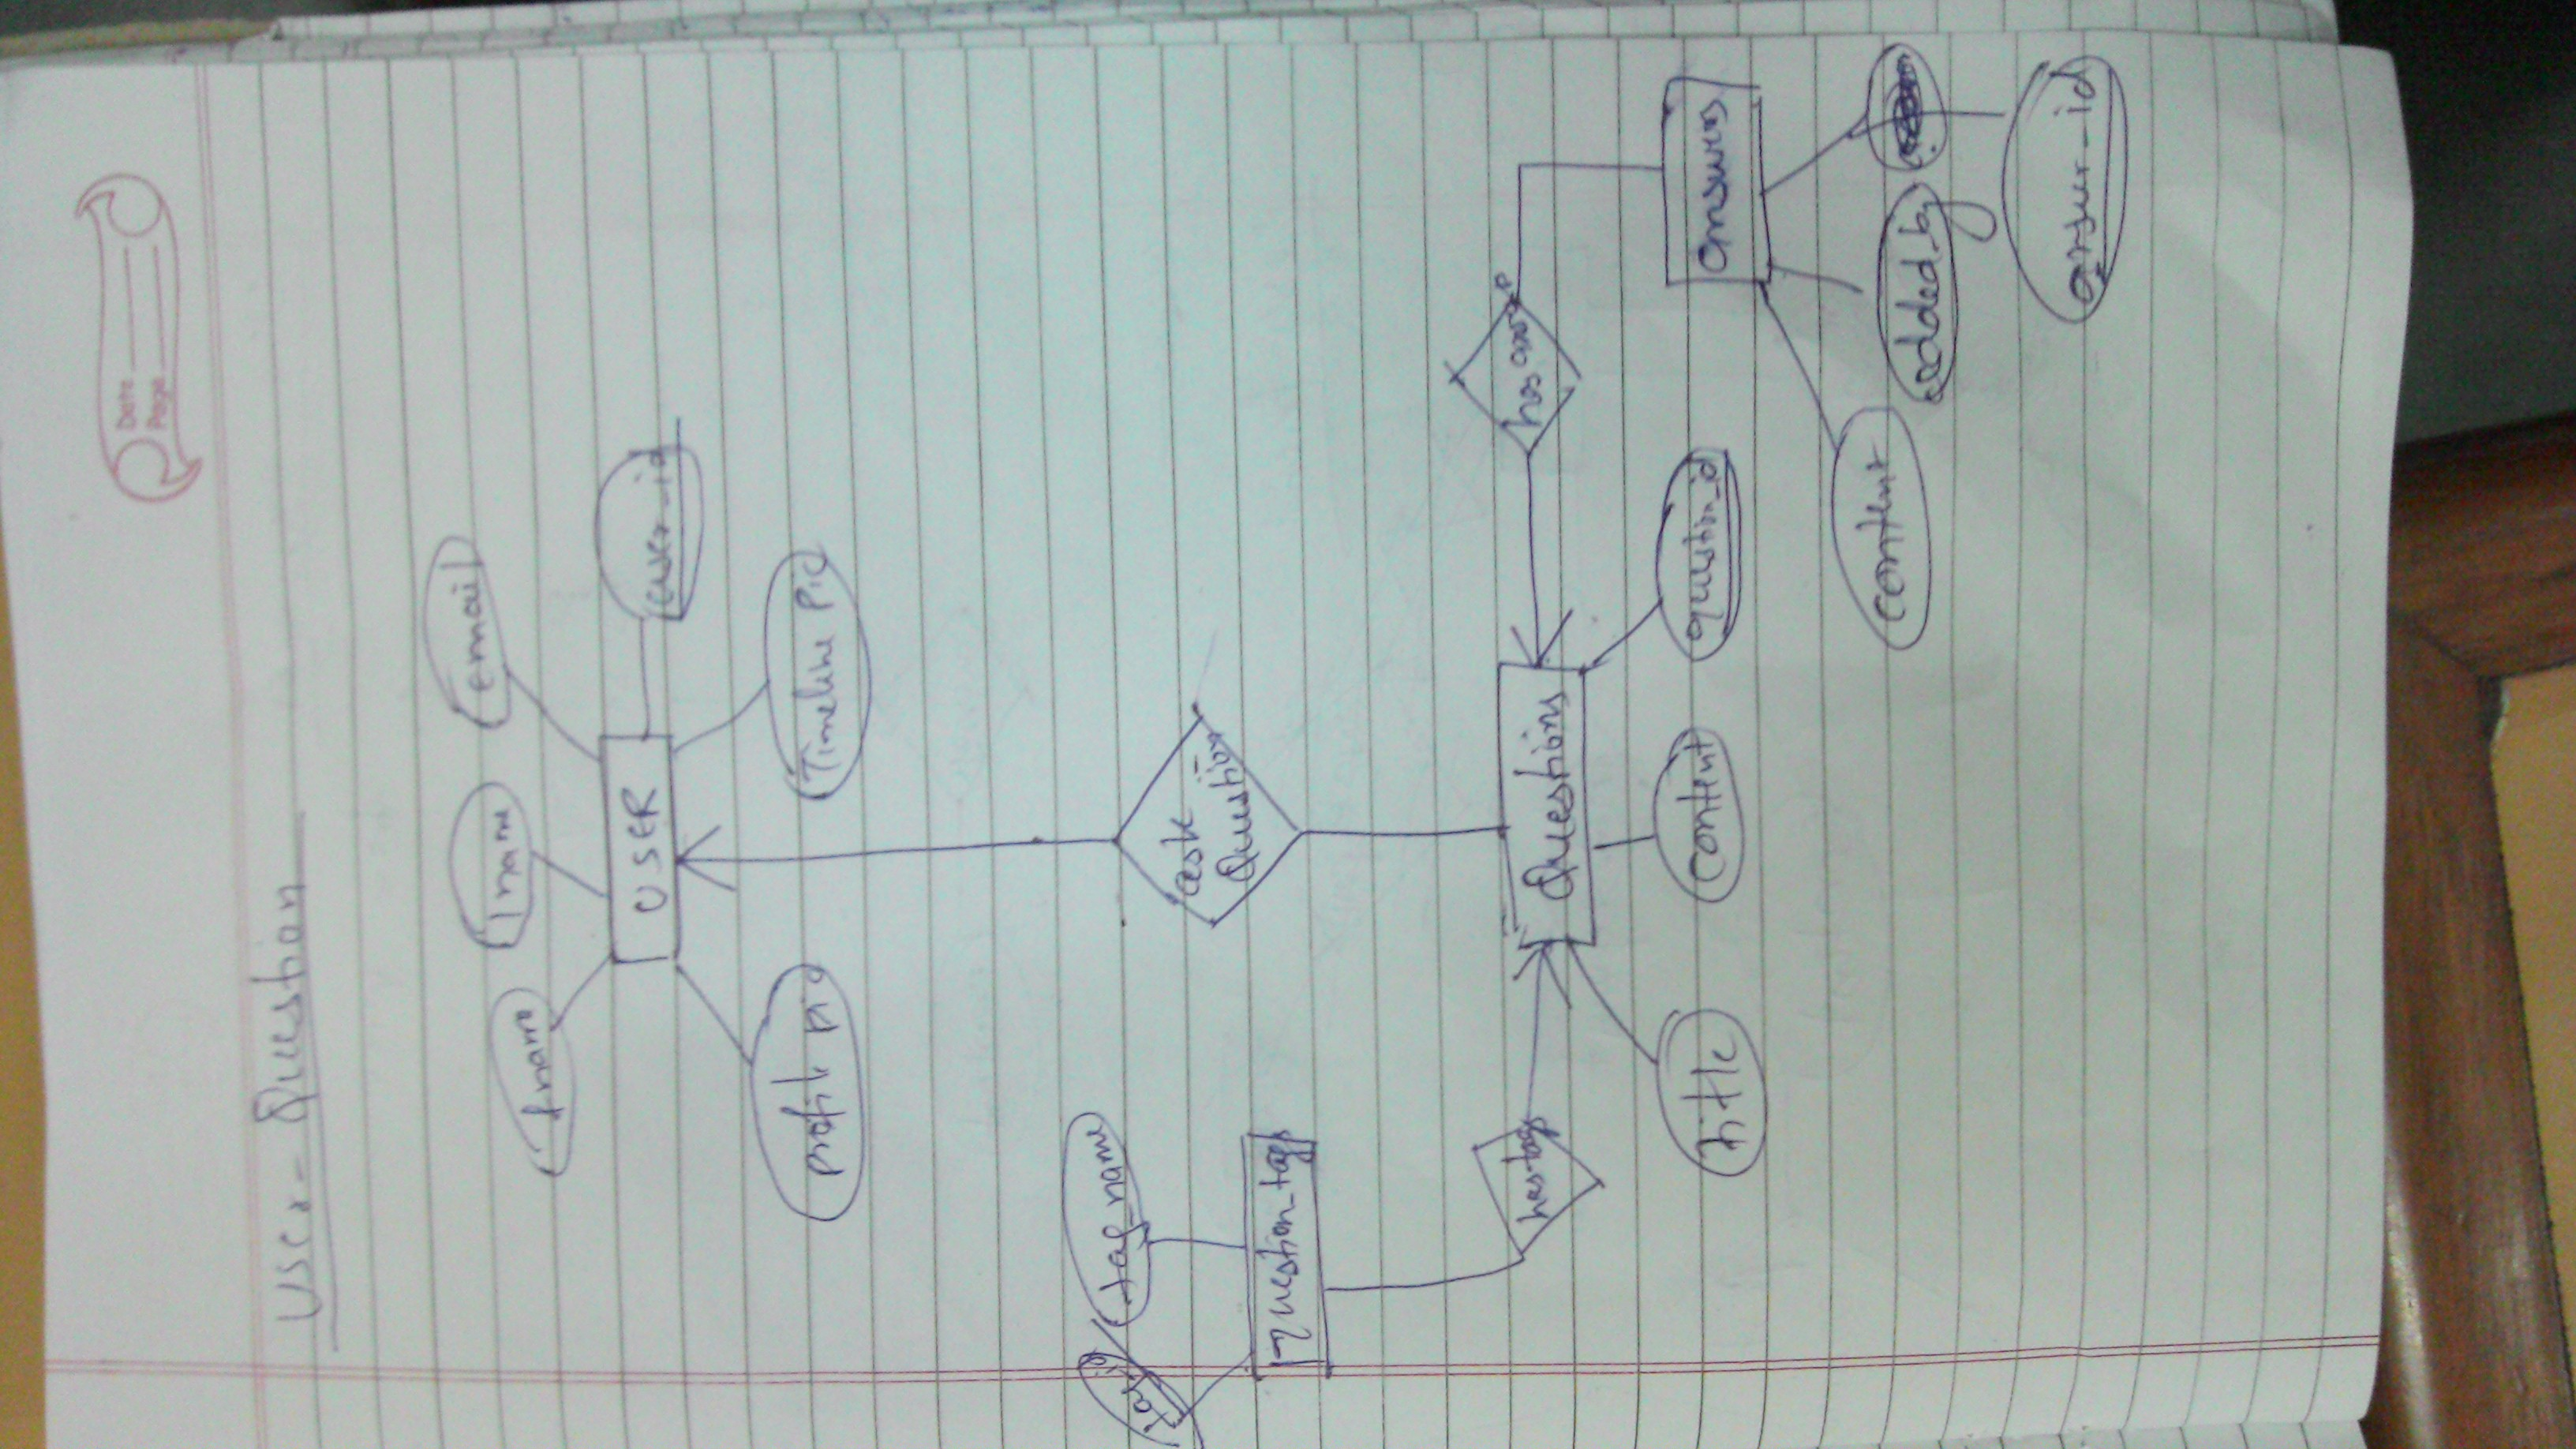
\includegraphics[scale=0.2]{fig4.jpg}
\caption{User - Question relation}
\label{fig4}
\end{figure}
Apart from pages and groups, a platform is provided to all users to ask question which will be visible to everyone and any user can answer to anyone's query. Users can even search for questions, if already asked by other users and find their answers. User - Question relation can be described as follows:
\begin{itemize}
\item \textbf{Ask questions:} User can ask any question which would be visible to everybody to answer. A question will have attributes - question title, content.
\item \textbf{Has answers:} A question can have multiple answers from multiple users. An answer will contain a content and the user who added that answer.
\item \textbf{Question-tags:} In order to optimize the search query, each question will have certain tags added by user who asked that question. 
\end{itemize} 
\subsection{User - Wall relation}
\begin{figure}[h]
\centering
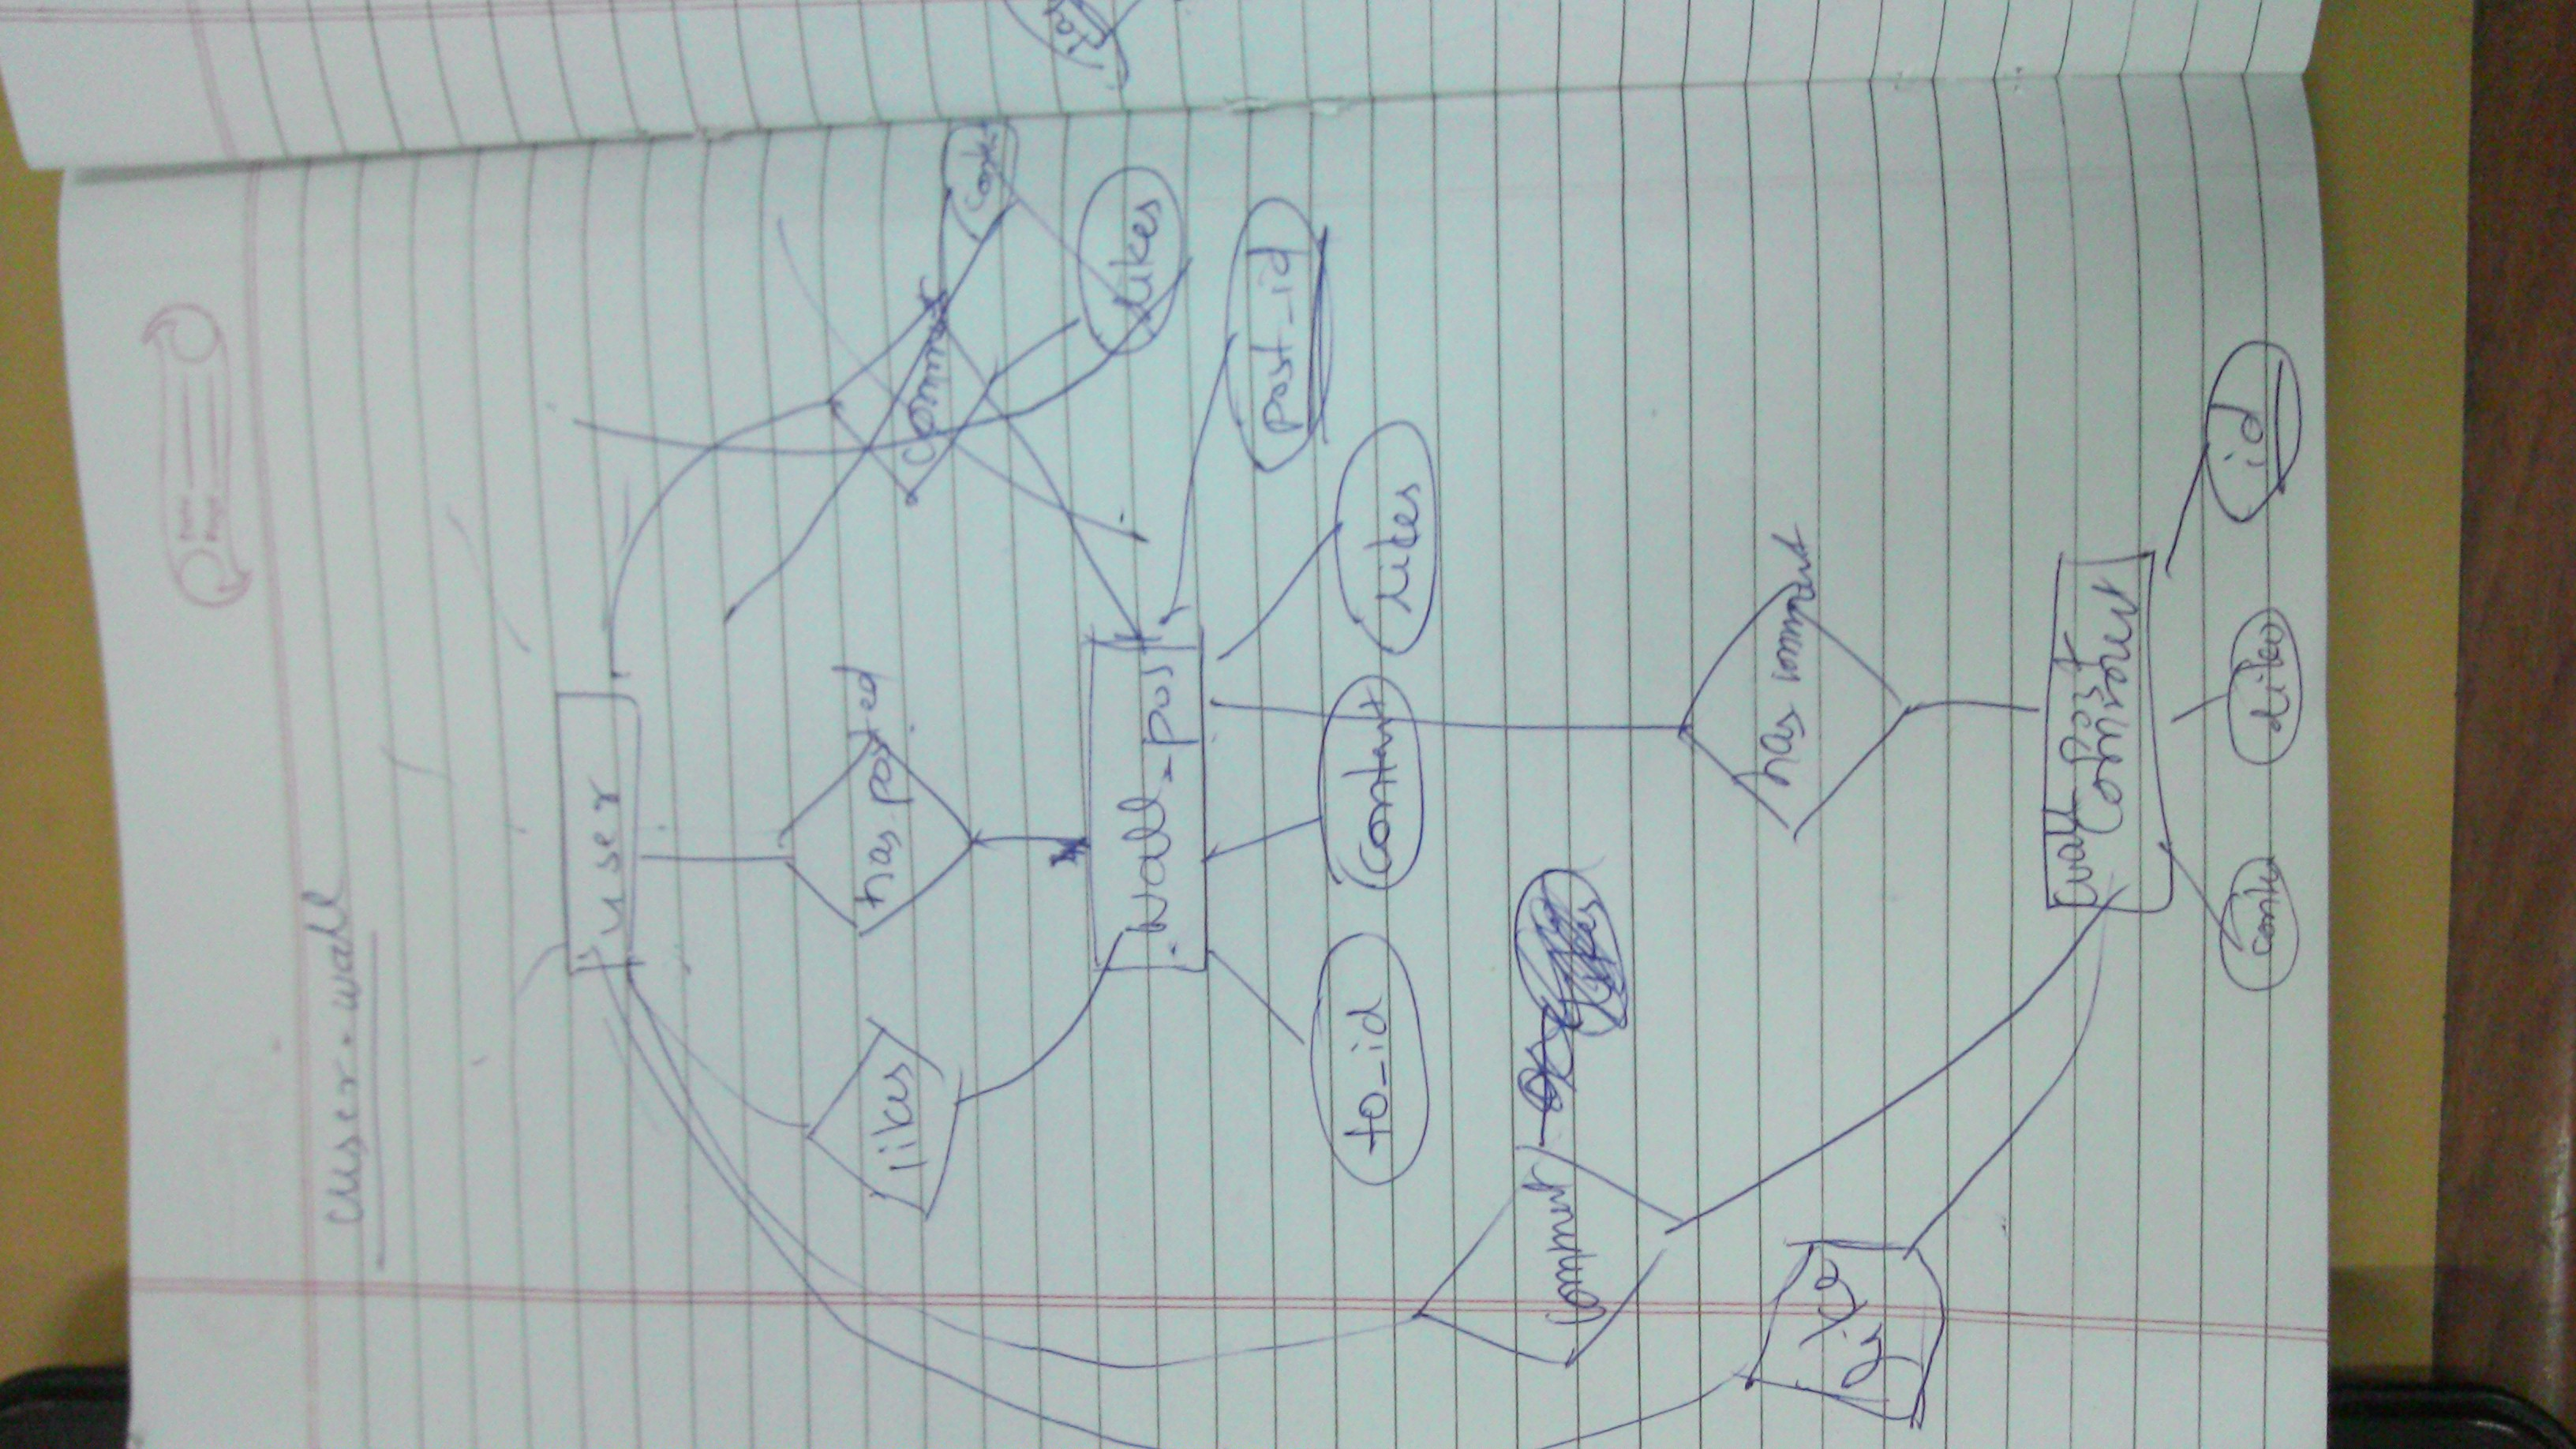
\includegraphics[scale=0.2]{fig5.jpg}
\caption{User - Wall relation}
\label{fig5}
\end{figure}
Each user has certain area on his profile, which we call, $wall$, where his/her friends can post or comments. User or his/her friends can like each others post or comments on each other walls. User can interact with walls in following way:
\begin{itemize}
\item \textbf{Wall post:} A user can post to his/her own wall or on the walls of his/her friends. Each post has attributes: content, user on whose wall it is posted, number of likes on the post etc.
\item \textbf{Wall comment:} Users can even comment on the posts by other users which will have same attributes as posts.
\item \textbf{Like post/comment:} A user can like any posts and comments. 
\end{itemize}
\subsection{User - Message relation}
\begin{figure}[h]
\centering
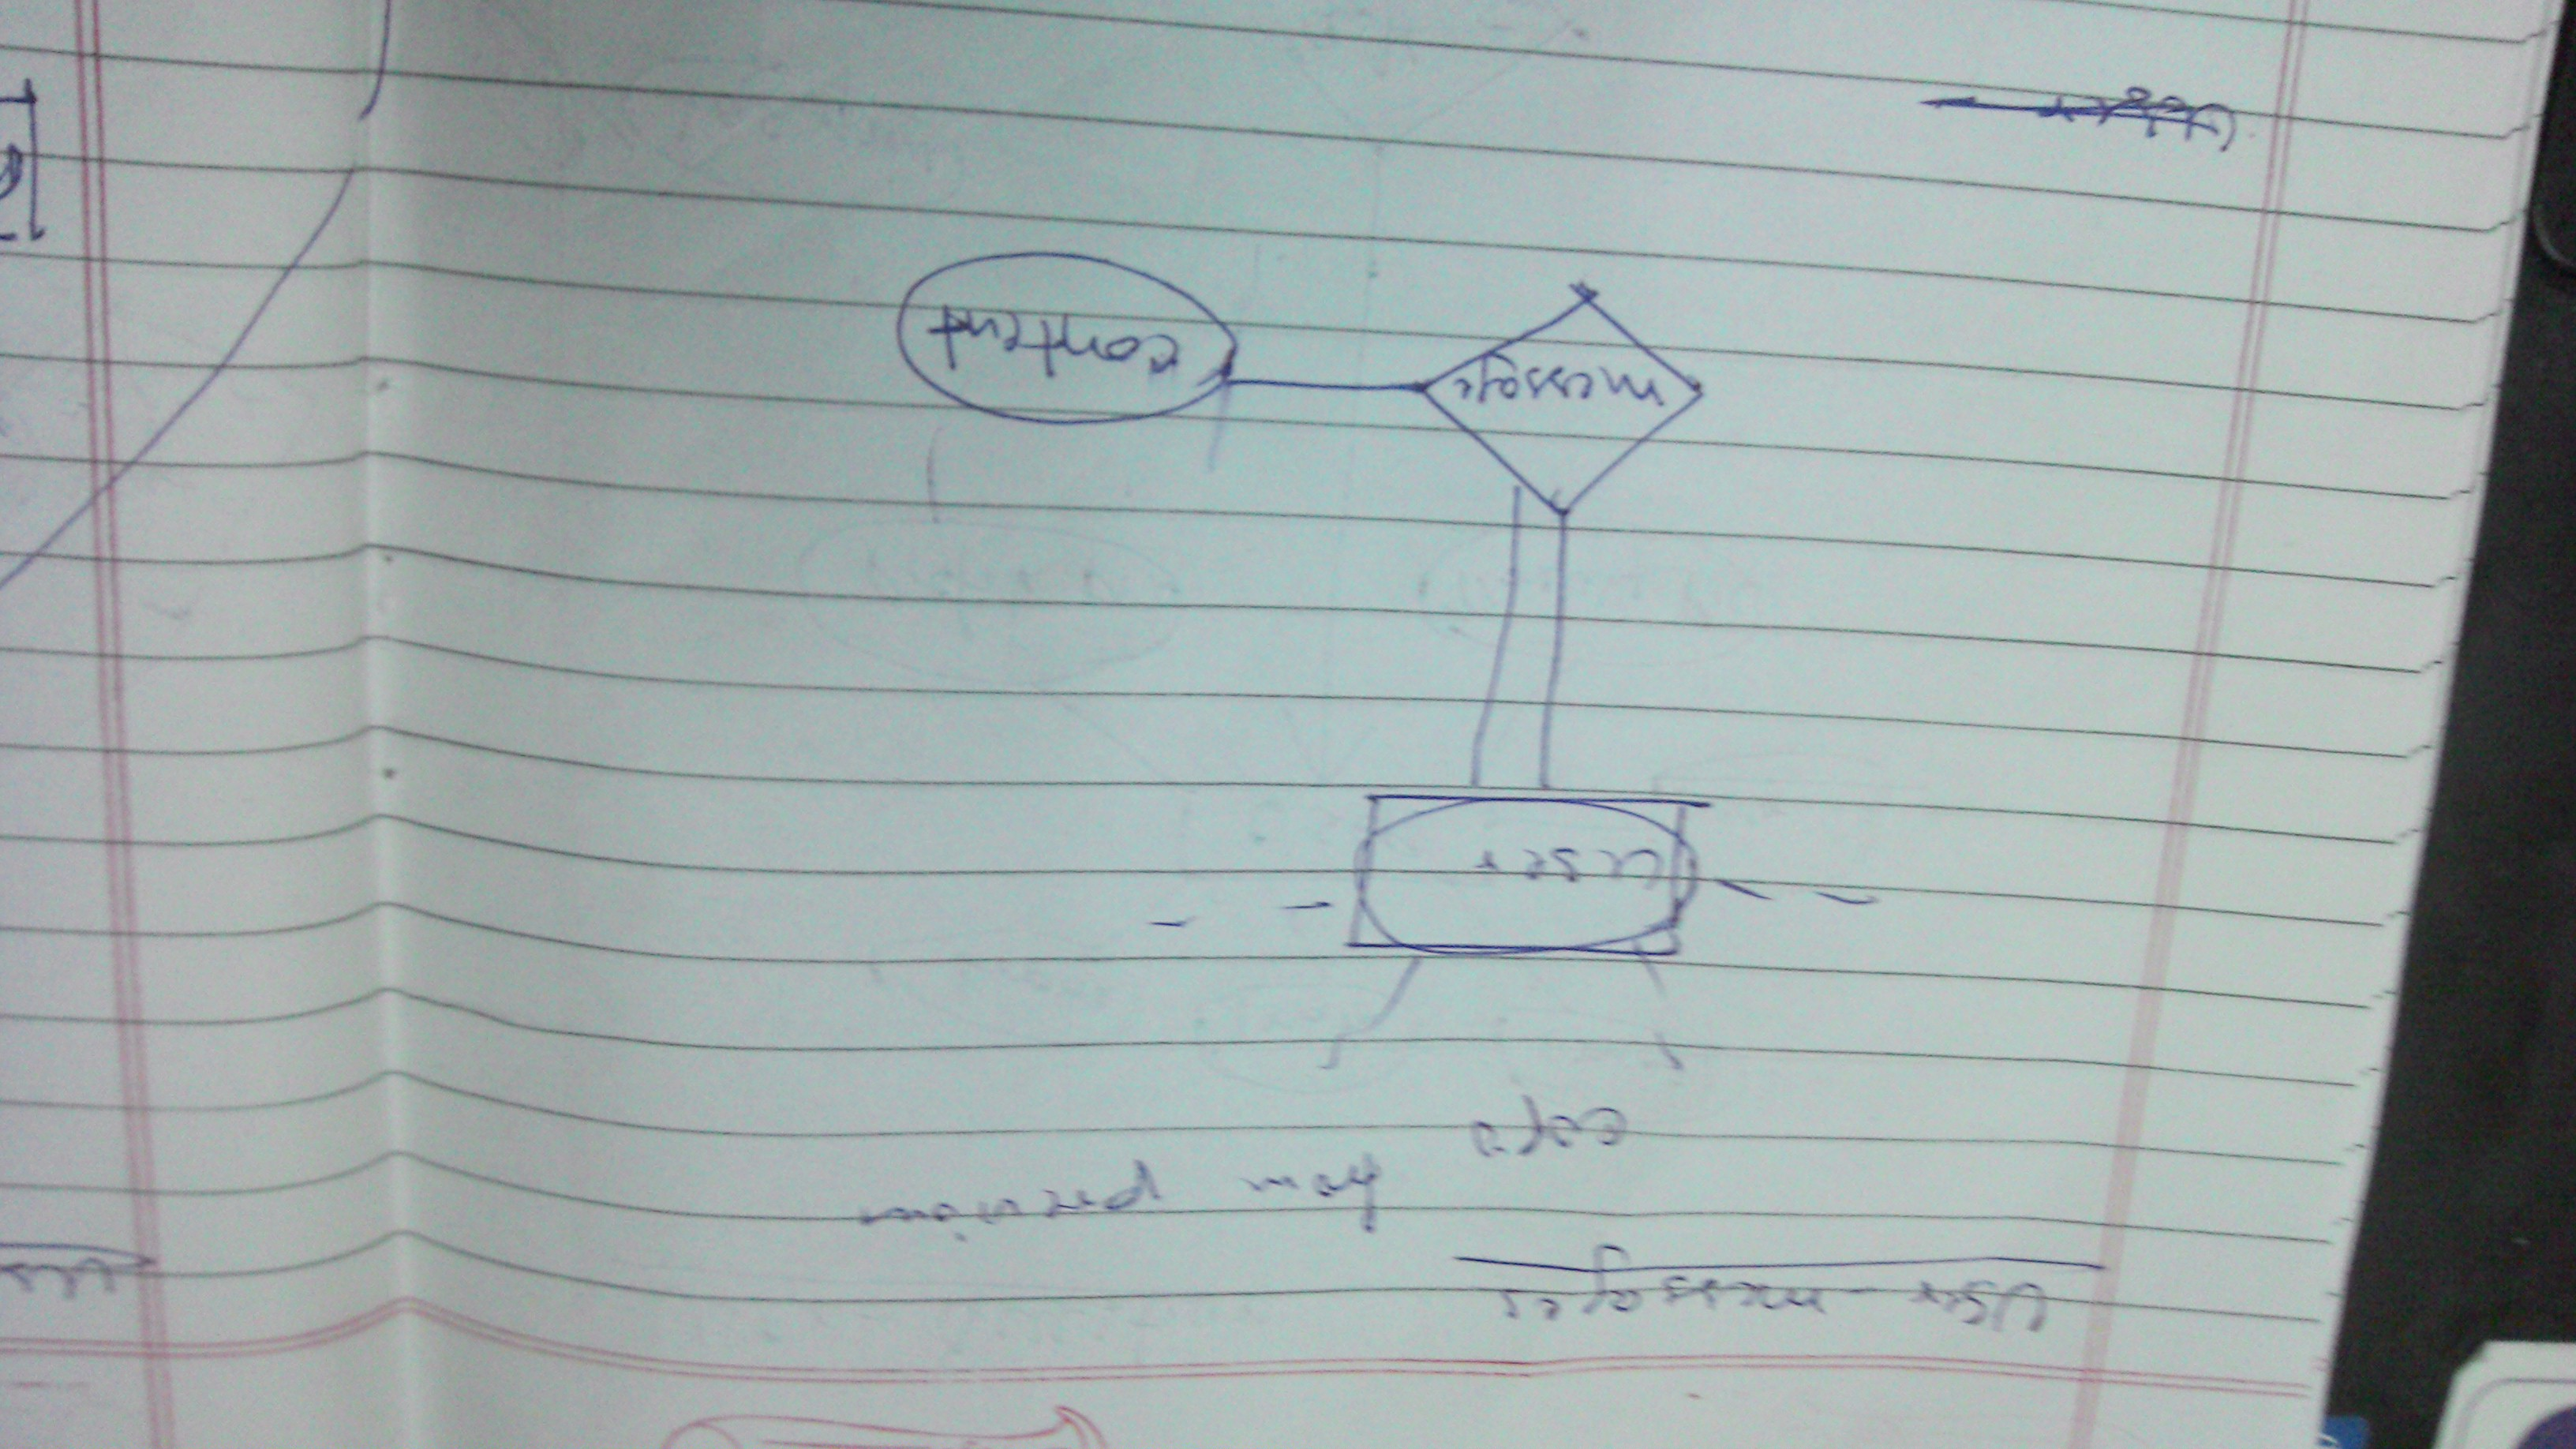
\includegraphics[scale=0.2]{fig6.jpg}
\caption{User - Message relation}
\label{fig6}
\end{figure}
Another interesting feature of the social network is the instant messaging. Users can communicate with each other privately using chat and it will store all the previous conversations. Each message will have some content and only two users can be related through messages.

\section{Features}
\subsection{Security measures}
\begin{itemize}
\item \textbf{Email verification:} At the time of registering new users, we need their email address of the user in order to verify their identity. When users sign up , they automatically receive an email request to verify their address. To verify, they just need to click on the link in the message. This veriifcation link is generated using 15 hexadecimal of random number which is stored in the database for verification.
\item \textbf{Cookies protection:} Since cookies hold sensitive session information, they need to be verified each time they are used in order to ensure that they have not been tampered. Each time a user login, we store following cookies in the browser:
\begin{itemize}
\item username: Name of the user logged in
\item userid: The id of the user, which acts as primary key.
\item checksum: A 15 hexadecimal long random number
\end{itemize}
userid and checksum is also stored in the database on server side and everytime cookies are used, checksum stored in the browser is matched with that stored in the database. If matching fails, user is logged out immediately and need to login again, otherwise, required action is executed. This ensures integrality of cookies. 
\item \textbf{Groups privacy:} Since, groups can be private, a non-member is not allowed to view the content of the group unless his request to join group is accepted by the creator of the group.
\end{itemize}
\section{Future work}

\section{References}
\end{document}